% !TeX root = Main.tex

\renewcommand\thepage{}
\begin{figure}[!h]
	\centering
	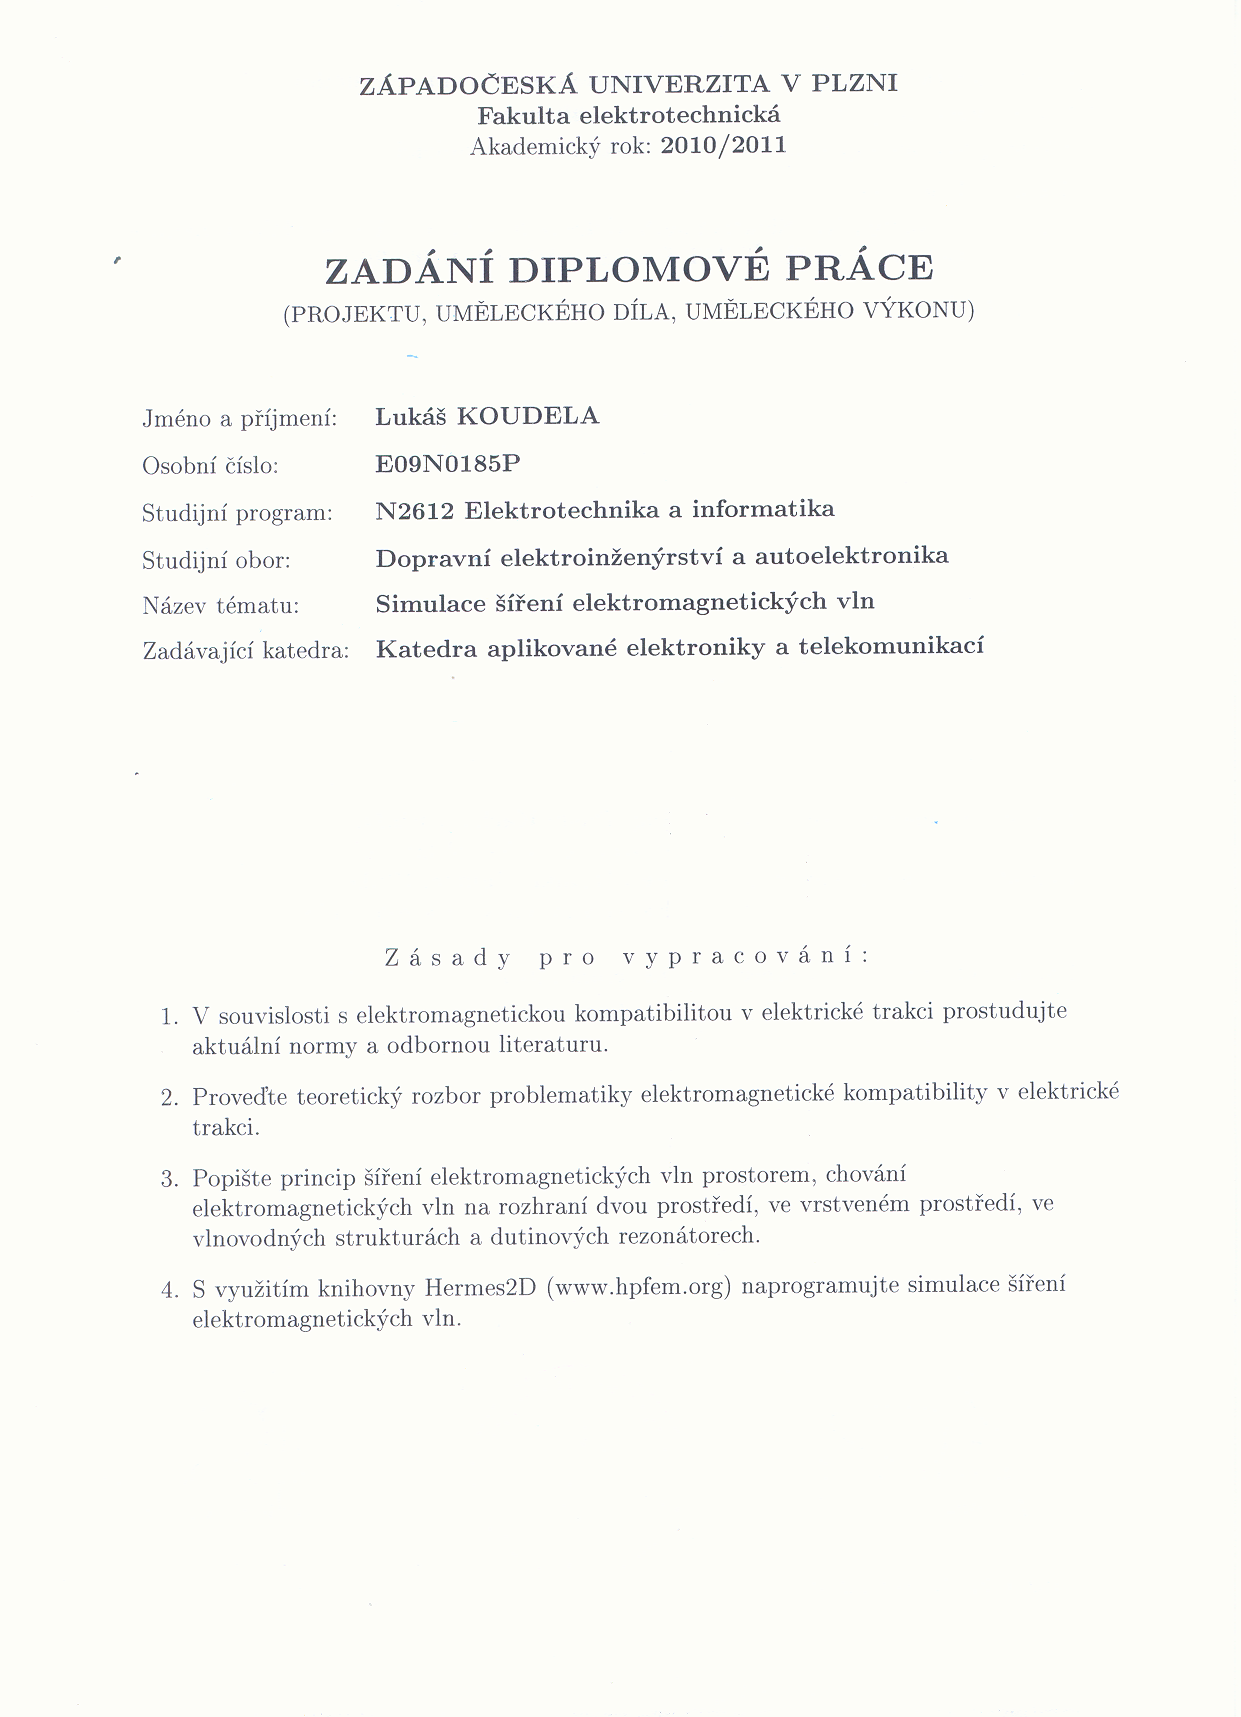
\includegraphics[width=15cm]{zadani1.png}
\end{figure}
\titlepage
\begin{figure}[!h]
	\centering
	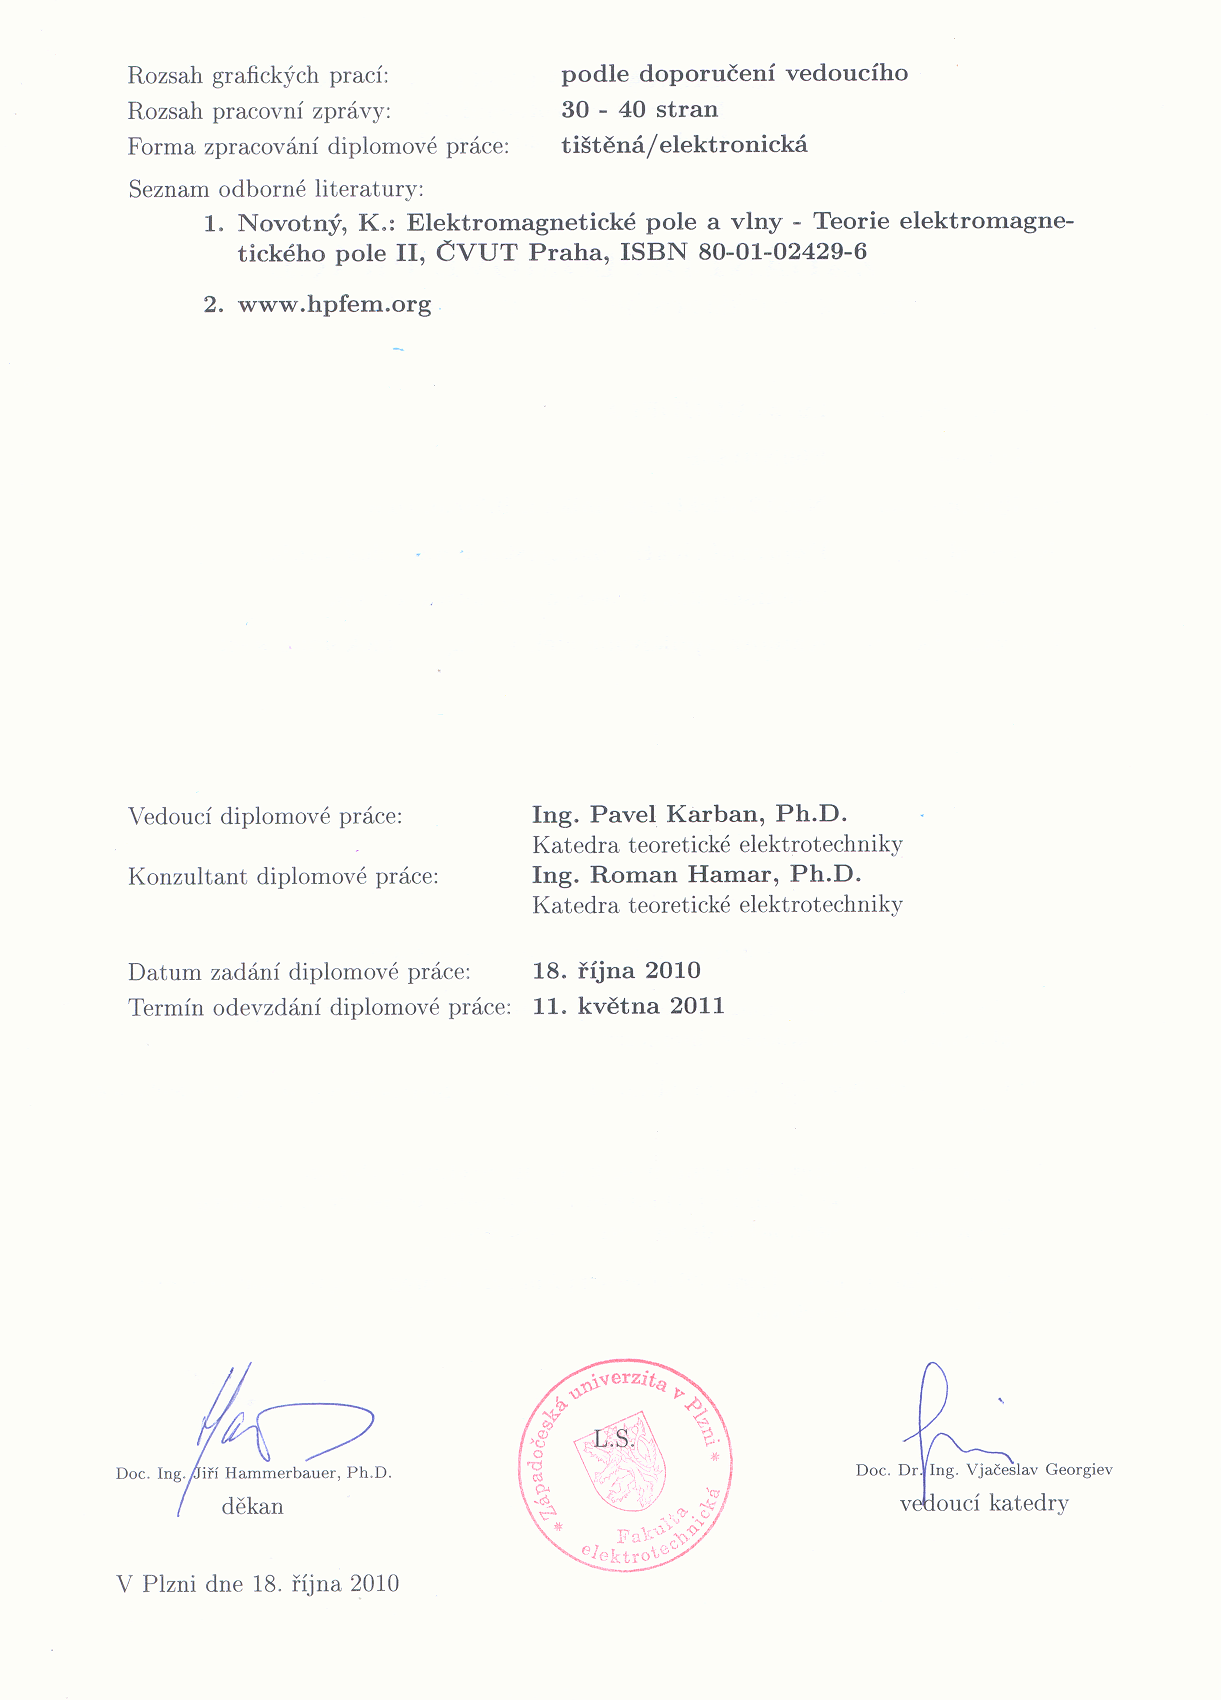
\includegraphics[width=15cm]{zadani2.png}
\end{figure}
\newpage

\section*{Anotace}
Předložená diplomová práce se zabývá principem šíření elektromagnetických vln. Hlavní cíl práce představuje realizace softwarové aplikace s~využitím knihovny Hermes2D.

Úzce pojednává o~problematice elektromagnetické kompatibility v~elektrické trakci a uvádí související normy. Dále je uveden popis chování vln v~různých prostředích a jsou sestaveny příslušné diferenciální rovnice, které jsou následně použity k~tvorbě simulačního modulu.  Nakonec je rozdebrána vlastní praktická část, tvorba software a popis jeho použití na simulaci úlohy z~oboru vysokofrekvenční techniky.

\section*{Klíčová slova}
EMC, elektrická trakce, programovací jazyk C++, metoda konečných prvků, okrajové podmínky, Hermes2D, Agros2D

\bigskip
% The Simulation of Electromagnetic Wales Propagation

\section*{Annotation}
The present thesis deals with the principle of electromagnetic waves propagation. The main goal is to build of software application with the use the library Hermes2D.

The thesis is divided into three main parts. Firstly, it discusses closely the issues of electromagnetic compatibility in electric traction and provides related standards.
In the next part is the behavior of waves in different environments decribed and the relevant differential equations for the simulation are formulated. The third part deals with the implementation of software and describes its application to task of RF field.

\section*{Keywords}
EMC, Electric traction, programming language C++, finite element method, boundary conditions, Hermes2D, Agros2D
\newpage

\section*{Prohlášení}
Předkládám tímto k~posouzení a obhajobě diplomovou práci zpracovanou na závěr studia na Fakultě elektrotechnické Západočeské univerzity v~Plzni.

\hyphenation{literatury}
Prohlašuji, že jsem diplomovou práci vypracoval samostatně s~použitím odborné literatury a pramenů uvedených v~seznamu, který je součástí této diplomové práce.
Dále prohlašuji, že veškerý software, použitý při řešení této diplomové práce, byl využit s~respektováním všech jeho licenčních podmínek.\bigskip \bigskip \\

\noindent V~Plzni, dne 3. května 2011 \hfill \ldots \ldots \ldots \ldots \ldots \ldots \ldots \ldots \ldots \ldots
\noindent \begin{flushright}Bc. Lukáš Koudela ~~~~~~~\end{flushright}
\newpage

\section*{Poděkování}
Na tomto místě bych rád vyjádřit poděkování vedoucímu diplomové práce Ing. Pavlu Karbanovi, Ph.D. za veškeré cenné rady, konstruktivní připomínky, ochotu a čas, který mi při řešení problémů spojených s~touto prací věnoval.

\hyphenation{Mlsnové}
Také bych touto cestou chtěl poděkovat svým rodičům a přítelkyni Stanislavě Mlsnové za veškerou jejich nedocenitelnou podporu během studia. Bez jejich pomoci by tato práce nikdy nevznikla.\bigskip \bigskip \\

\noindent V~Plzni, dne 3. května 2011 \hfill \ldots \ldots \ldots \ldots \ldots \ldots \ldots \ldots \ldots \ldots
\noindent \begin{flushright}Bc. Lukáš Koudela ~~~~~~~\end{flushright}
\newpage